
\chapter{Introducción}

En este capítulo se presenta el estado del arte relacionado con la
identificación de variedades de vid mediante características foliares, así
como la problemática que motiva el desarrollo del proyecto, su
justificación, objetivos, hipótesis y metodología propuesta. La revisión
comprende desde los métodos ampelográficos tradicionales hasta las técnicas
actuales basadas en aprendizaje profundo y su implementación en dispositivos
con recursos computacionales limitados.

\section{Estado del Arte}

Esta sección presenta el estado del arte mediante una revisión sistemática de
la literatura. La ejecución de la revisión sigue los lineamientos de
Kitchenham y Charters \citep{kitchenham2007}, mientras que la documentación
del proceso de búsqueda y selección se apega al protocolo PRISMA 2020
\citep{page2021prisma}.

\subsection{Metodología de la revisión sistemática}

\subsubsection{Justificación de la revisión}

La identificación de variedades de vid (\textit{Vitis vinifera} L.) mediante
el análisis de hojas ha evolucionado desde la ampelografía tradicional hasta
el uso de redes neuronales convolucionales, pasando por descriptores
morfométricos y clasificadores de aprendizaje automático. Sin embargo, los
estudios reportados emplean conjuntos de datos, arquitecturas, métricas y
condiciones de evaluación heterogéneas, lo que dificulta determinar qué
enfoques ofrecen un mejor equilibrio entre exactitud de clasificación y
viabilidad de implementación en plataformas embebidas. Por esta razón se
plantea una revisión sistemática que permita identificar, organizar y
comparar la evidencia disponible sobre algoritmos, conjuntos de datos y
estrategias de generalización e implementación embebida aplicadas a la
identificación varietal de vid mediante hojas.

\subsubsection{Preguntas de investigación}

\begin{itemize}
    \item \textbf{PI1.} ¿Qué algoritmos y arquitecturas se han utilizado para
    clasificar variedades de vid a partir de imágenes de hojas?
    \item \textbf{PI2.} ¿Qué conjuntos de datos (públicos o propios) se han
    empleado, y qué variedades y cantidad de imágenes cubren?
    \item \textbf{PI3.} ¿Qué métricas y niveles de desempeño se han reportado
    para estos clasificadores?
    \item \textbf{PI4.} ¿Cómo se ha evaluado la capacidad de generalización de
    los modelos frente a datos externos al entrenamiento?
    \item \textbf{PI5.} ¿Qué estrategias se han utilizado para implementar
    estos modelos en dispositivos con recursos computacionales limitados?
\end{itemize}

\subsubsection{Estrategia de búsqueda}

La estrategia de búsqueda se diseñó en dos fases. La \textbf{Fase~1}, cuyos
resultados se reportan en esta revisión, consistió en la ejecución de las
cadenas de búsqueda sobre fuentes de acceso abierto y motores académicos de
cobertura amplia, complementada con el rastreo de referencias
(\textit{snowballing}) de los estudios recuperados. La \textbf{Fase~2}, que
se ejecutará mediante el acceso institucional de la Universidad Autónoma de
Baja California, replicará las mismas cadenas en Scopus, Web of Science e
IEEE Xplore para incorporar los registros no accesibles públicamente. Esta
separación se documenta de manera explícita para que el proceso sea
reproducible y para distinguir con claridad el alcance de la evidencia aquí
sintetizada.

\paragraph{Fuentes de información}

La búsqueda de la Fase~1 se realizó en las fuentes listadas en la
Tabla~\ref{tab:fuentes}, seleccionadas por su cobertura en agricultura de
precisión, visión por computadora, aprendizaje profundo e ingeniería
electrónica, así como por la disponibilidad de texto completo. Se
consideraron publicaciones en inglés y español desde el año 2001 —fecha del
primer antecedente morfométrico cuantitativo identificado— hasta septiembre
de 2026. La última búsqueda se ejecutó el \textbf{17 de septiembre de 2026}.
Los registros se consolidaron en una hoja de extracción única, en la que se
eliminaron los duplicados comparando título, autores y DOI.

\begin{longtable}{L{4.6cm}L{2.8cm}L{2.6cm}L{3.2cm}}
\caption{Fuentes de información consultadas en la Fase~1 de la búsqueda.}
\label{tab:fuentes} \\
\toprule
\textbf{Fuente} & \textbf{Fecha de búsqueda} & \textbf{Periodo} & \textbf{Registros recuperados} \\
\midrule
\endfirsthead
\toprule
\textbf{Fuente} & \textbf{Fecha de búsqueda} & \textbf{Periodo} & \textbf{Registros recuperados} \\
\midrule
\endhead
Motor académico general (Google Scholar y buscador web indexado) & 17/09/2026 & 2001--2026 & 32 \\
ScienceDirect (Elsevier) & 17/09/2026 & 2001--2026 & 8 \\
MDPI (\textit{Plants}, \textit{Agriculture}, \textit{Sensors}, \textit{AgriEngineering}) & 17/09/2026 & 2018--2026 & 6 \\
SpringerLink & 17/09/2026 & 2015--2026 & 6 \\
IEEE Xplore (acceso público) & 17/09/2026 & 2015--2026 & 3 \\
Otras fuentes revisadas por pares (Cambridge Core, PLOS ONE, Frontiers, Nature Portfolio, Acta Horticulturae) & 17/09/2026 & 2019--2026 & 7 \\
Repositorios de datos y preimpresiones (Zenodo, Kaggle, arXiv) & 17/09/2026 & 2021--2026 & 3 \\
\midrule
\textbf{Total} & & & \textbf{65} \\
\bottomrule
\end{longtable}

\paragraph{Palabras clave}

Los conceptos principales derivados de las preguntas de investigación y sus
sinónimos se presentan en la Tabla~\ref{tab:palabras}. Se incluyeron términos
en inglés por ser el idioma predominante de la literatura especializada.

\begin{longtable}{L{3.6cm}L{10.4cm}}
\caption{Conceptos y palabras clave utilizadas en las cadenas de búsqueda.}
\label{tab:palabras} \\
\toprule
\textbf{Concepto} & \textbf{Palabras clave y sinónimos} \\
\midrule
\endfirsthead
\toprule
\textbf{Concepto} & \textbf{Palabras clave y sinónimos} \\
\midrule
\endhead
Vid / uva & ``grapevine'', ``grape'', ``Vitis vinifera'', ``cultivar'' \\
Hoja & ``leaf'', ``leaves'', ``foliar'' \\
Identificación de variedad & ``variety identification'', ``variety classification'', ``cultivar classification'', ``cultivar identification'', ``ampelography'' \\
Aprendizaje profundo & ``deep learning'', ``convolutional neural network'', ``CNN'', ``transfer learning'', ``vision transformer'' \\
Conjunto de datos & ``dataset'', ``image dataset'', ``benchmark'' \\
Generalización & ``generalization'', ``robustness'', ``domain shift'', ``external validation'' \\
Sistema embebido & ``embedded system'', ``edge computing'', ``edge device'', ``lightweight model'', ``mobile deployment'' \\
\bottomrule
\end{longtable}

\paragraph{Cadenas de búsqueda}

Se ejecutaron siete cadenas de búsqueda derivadas de la combinación de los
conceptos anteriores. Las tres cadenas principales se muestran a
continuación.

Cadena general:
\begin{verbatim}
("grapevine" OR "grape" OR "Vitis vinifera" OR cultivar)
AND
(leaf OR leaves OR foliar)
AND
("variety identification" OR "variety classification" OR
 "cultivar classification" OR ampelography)
AND
("deep learning" OR "convolutional neural network" OR CNN
 OR "machine learning")
\end{verbatim}

Cadena enfocada en implementación embebida:
\begin{verbatim}
("grapevine" OR "Vitis vinifera") AND (leaf OR foliar)
AND ("embedded system" OR "edge computing" OR
     "lightweight model" OR "mobile application"
     OR "edge device")
\end{verbatim}

Cadena enfocada en generalización y conjuntos de datos:
\begin{verbatim}
("grapevine" OR "grape") AND (leaf OR leaves)
AND (dataset OR benchmark)
AND (generalization OR robustness OR "domain shift"
     OR "external validation")
\end{verbatim}

Durante la ejecución fue necesario adaptar las cadenas a la sintaxis de cada
fuente. En los motores académicos generales se eliminaron los paréntesis
anidados, que no son soportados, y cada bloque conceptual se ejecutó como una
consulta independiente cuyos resultados se unieron manualmente. En MDPI y
SpringerLink las comillas dobles se conservaron pero el operador \texttt{AND}
se sustituyó por la búsqueda por campos de título y resumen. En ScienceDirect
se aplicó además el filtro de tipo de documento ``research article'' para
descartar editoriales y capítulos introductorios.

\subsubsection{Criterios de inclusión y exclusión}

\textbf{Criterios de inclusión}
\begin{itemize}
    \item Estudios sobre identificación o clasificación de variedades de vid
    (\textit{Vitis vinifera}) mediante hojas.
    \item Investigaciones que describan un método ampelográfico, morfométrico,
    de aprendizaje automático o aprendizaje profundo.
    \item Estudios que utilicen conjuntos de datos de imágenes foliares,
    públicos o propios.
    \item Conjuntos de datos públicos de imágenes de hoja de vid etiquetados
    por variedad, incorporados como recursos de datos.
    \item Artículos publicados en revistas o congresos con revisión por pares.
    \item Publicaciones en inglés o español dentro del periodo establecido.
    \item Documentos con texto completo disponible.
\end{itemize}

\textbf{Criterios de exclusión}
\begin{itemize}
    \item Registros duplicados.
    \item Estudios sobre otras especies vegetales sin relación directa con vid,
    o sobre órganos distintos de la hoja (semilla, baya, sarmiento).
    \item Estudios enfocados exclusivamente en detección de enfermedades sin
    relación con identificación varietal. Estos se documentan como antecedente
    narrativo cuando aportan evidencia sobre arquitecturas ligeras o
    implementación embebida, pero no se integran a la extracción formal.
    \item Revisiones, editoriales, resúmenes y presentaciones sin datos
    originales.
    \item Propuestas teóricas sin implementación ni evaluación experimental.
    \item Documentación técnica, tutoriales y repositorios de código sin
    revisión por pares.
    \item Documentos no recuperados a texto completo o publicados fuera del
    periodo establecido.
\end{itemize}

\subsubsection{Proceso de selección}

Los registros recuperados de las siete cadenas se integraron en una hoja de
extracción única. Primero se eliminaron los duplicados comparando título,
autores y DOI; posteriormente se cribaron títulos y resúmenes aplicando los
criterios de elegibilidad, y finalmente los documentos potencialmente
relevantes se recuperaron y evaluaron a texto completo. Las cifras del
proceso se presentan en la Tabla~\ref{tab:seleccion} y el flujo completo en
la Figura~\ref{fig:prisma}.

\begin{longtable}{L{9.5cm}L{3.5cm}}
\caption{Resultados del proceso de selección de estudios (Fase~1).}
\label{tab:seleccion} \\
\toprule
\textbf{Etapa} & \textbf{Cantidad} \\
\midrule
\endfirsthead
\toprule
\textbf{Etapa} & \textbf{Cantidad} \\
\midrule
\endhead
Registros identificados & 65 \\
Duplicados eliminados & 18 \\
Registros cribados (título/resumen) & 47 \\
Registros excluidos en el cribado & 27 \\
Informes buscados a texto completo & 20 \\
Informes no recuperados (acceso restringido) & 2 \\
Informes evaluados a texto completo & 18 \\
Informes excluidos a texto completo & 6 \\
Registros retenidos en la Fase~1 & 12 \\
\quad Coincidentes con la revisión narrativa previa & 5 \\
\quad Nuevos registros incorporados & 7 \\
\midrule
\textbf{Total de registros incluidos en la revisión} & \textbf{26} \\
\bottomrule
\end{longtable}

El corpus final está formado por los 19 registros documentados en la revisión
narrativa previa del proyecto más los 7 registros nuevos aportados por la
Fase~1, para un total de 26 registros incluidos (22 estudios y 4 recursos de
datos).

\begin{figure}[htbp]
\centering
\begin{tikzpicture}[
    node distance=7mm and 10mm,
    box/.style={rectangle, draw=blue!60!black, fill=blue!8, rounded corners,
        text width=5.2cm, align=center, minimum height=1.0cm, font=\small},
    sidebox/.style={rectangle, draw=blue!40!black, fill=blue!4, rounded corners,
        text width=5.8cm, align=left, minimum height=1.0cm, font=\footnotesize},
    hdr/.style={rectangle, draw=blue!70!black, fill=blue!70!black, text=white,
        text width=5.2cm, align=center, minimum height=0.8cm, font=\small\bfseries},
    arr/.style={-{Latex[length=2mm]}, thick, draw=blue!60!black}
]

\node[hdr] (hdr1) {Identificación de estudios mediante bases de datos y registros};

\node[box, below=of hdr1] (identificados)
    {Registros identificados\\en las fuentes consultadas\\(n = 65)};
\node[sidebox, right=of identificados] (eliminados)
    {Registros eliminados antes del cribado:\\
     Duplicados eliminados (n = 18)\\
     Marcados no elegibles por automatización (n = 0)\\
     Eliminados por otras razones (n = 0)};

\node[box, below=of identificados] (cribados)
    {Registros cribados\\(n = 47)};
\node[sidebox, right=of cribados] (excluidos1)
    {Registros excluidos\\(n = 27)};

\node[box, below=of cribados] (buscados)
    {Informes buscados para\\su recuperación\\(n = 20)};
\node[sidebox, right=of buscados] (norecuperados)
    {Informes no recuperados\\por acceso restringido (n = 2)};

\node[box, below=of buscados] (elegibilidad)
    {Informes evaluados para\\determinar su elegibilidad\\(n = 18)};
\node[sidebox, right=of elegibilidad] (excluidos2)
    {Informes excluidos (n = 6):\\
     Enfermedades sin relación varietal (n = 3)\\
     Revisión sin datos originales (n = 1)\\
     Órgano distinto de la hoja (n = 1)\\
     Sin relación con lo varietal (n = 1)};

\node[box, below=of elegibilidad] (retenidos)
    {Registros retenidos en la Fase~1 (n = 12)\\
     Nuevos (n = 7); ya documentados (n = 5)};

\node[box, below=of retenidos] (incluidos)
    {Registros incluidos en la revisión (n = 26)\\
     Estudios (n = 22); recursos de datos (n = 4)};

\draw[arr] (identificados) -- (cribados);
\draw[arr] (identificados) -- (eliminados);
\draw[arr] (cribados) -- (buscados);
\draw[arr] (cribados) -- (excluidos1);
\draw[arr] (buscados) -- (elegibilidad);
\draw[arr] (buscados) -- (norecuperados);
\draw[arr] (elegibilidad) -- (retenidos);
\draw[arr] (elegibilidad) -- (excluidos2);
\draw[arr] (retenidos) -- (incluidos);

\end{tikzpicture}
\caption{Diagrama de flujo del proceso de selección de estudios según PRISMA
2020, correspondiente a la Fase~1 de la búsqueda (17 de septiembre de 2026).}
\label{fig:prisma}
\end{figure}

\clearpage

\subsubsection{Evaluación de calidad}

La calidad metodológica de los estudios se evaluó mediante la rúbrica de
siete criterios presentada en la Tabla~\ref{tab:rubrica}. Se establece de
antemano que \textbf{la puntuación de calidad no se utiliza como criterio de
exclusión}, sino únicamente para ponderar la interpretación de la evidencia:
los hallazgos procedentes de estudios de calidad baja se reportan señalando
explícitamente esa condición.

\begin{longtable}{L{1.3cm}L{12.7cm}}
\caption{Rúbrica de evaluación de calidad metodológica.}
\label{tab:rubrica} \\
\toprule
\textbf{Código} & \textbf{Criterio de calidad} \\
\midrule
\endfirsthead
\toprule
\textbf{Código} & \textbf{Criterio de calidad} \\
\midrule
\endhead
C1 & ¿Se define claramente el objetivo de clasificación varietal? \\
C2 & ¿Se describe el conjunto de datos (variedades, tamaño, procedencia)? \\
C3 & ¿Se explica suficientemente la arquitectura o método utilizado? \\
C4 & ¿Se reportan métricas de desempeño (exactitud, F1, matriz de confusión)? \\
C5 & ¿Se evalúa la generalización mediante datos externos o independientes? \\
C6 & ¿Se abordan requerimientos computacionales o viabilidad embebida? \\
C7 & ¿Se discuten limitaciones o amenazas a la validez? \\
\bottomrule
\end{longtable}

Cada criterio se califica con 1 punto (sí), 0.5 (parcialmente) o 0 (no), para
un máximo de 7 puntos. Los niveles resultantes son: calidad alta, de 6 a 7
puntos; calidad media, de 4 a 5.5 puntos; y calidad baja, menos de 4 puntos.
Los cuatro recursos de datos (E14, E15, E16 y E26) no se puntúan, ya que la
rúbrica está diseñada para estudios experimentales.

\subsubsection{Extracción de datos}

La Tabla~\ref{tab:extraccion} contiene la hoja de extracción completa de los
26 registros incluidos. La columna de calidad reporta la puntuación obtenida
con la rúbrica C1--C7; se indica ``RD'' para los recursos de datos y ``NI''
(no informado) cuando el estudio no proporciona el dato correspondiente.

\begin{longtable}{L{0.7cm}L{2.5cm}L{3.3cm}L{2.6cm}L{2.4cm}L{0.6cm}}
\caption{Hoja de extracción de datos de los registros incluidos.}
\label{tab:extraccion} \\
\toprule
\textbf{ID} & \textbf{Referencia} & \textbf{Enfoque / Método} & \textbf{Variedades / Datos} & \textbf{Resultado principal} & \textbf{Cal.} \\
\midrule
\endfirsthead
\toprule
\textbf{ID} & \textbf{Referencia} & \textbf{Enfoque / Método} & \textbf{Variedades / Datos} & \textbf{Resultado principal} & \textbf{Cal.} \\
\midrule
\endhead
\midrule
\multicolumn{6}{r}{\footnotesize\textit{continúa en la página siguiente}} \\
\endfoot
\bottomrule
\endlastfoot
E01 & \citet{ates2011} & Descriptores ampelográficos + análisis de conglomerados & 10 cultivares (Turquía) & Diferenciación morfológica por conglomerados & 4.0 \\
E02 & \citet{mancuso2001} & Dimensión fractal (\textit{box-counting}) & Ecotipos de Sangiovese & Menor error que descriptores tradicionales & 3.0 \\
E03 & \citet{chitwood2014} & Morfometría geométrica (Fourier elíptico, Procrustes) & $>$1200 accesiones & Componentes genéticos de forma y venación & 4.5 \\
E04 & \citet{chitwood2020} & Integración de ampelografía clásica y morfometría & NI & Marco conceptual, sin clasificador automático & 2.0 \\
E05 & \citet{fuentes2018} & Morfo-colorimetría + fractal + NIR + ANN & 16 cultivares & Exactitud 94.2\% & 5.5 \\
E06 & \citet{koklu2022} & MobileNetV2 (extracción de características) + SVM & 5 variedades, 500 imágenes & Exactitud $>$97\% & 5.0 \\
E07 & \citet{reyes2015} & Ajuste fino de CNN preentrenadas & Reconocimiento de plantas (general) & Antecedente metodológico de transferencia & 3.5 \\
E08 & \citet{hall2015} & Evaluación de características para clasificación de hojas & Condiciones visuales complejas (general) & Antecedente metodológico, no específico de vid & 4.5 \\
E09 & \citet{pereira2019} & Transferencia de aprendizaje (AlexNet) & 6 variedades de uva tinta & Exactitud 77.3\% & 5.5 \\
E10 & \citet{liu2021} & Comparación de CNN + aplicación Android & 21 cultivares & Hasta 99.91\% (GoogLeNet); app funcional & 6.5 \\
E11 & \citet{magalhaes2023} & MobileNetV2 / ResNet-34 / VGG-11-BN & 26 variedades & F1-score 94.75\% (MobileNetV2) & 6.0 \\
E12 & \citet{terzi2024} & CNN con nuevas características ampelográficas & NI & Exactitud $\approx$94.1\% & 4.0 \\
E13 & \citet{adao2025} & Xception + Mask R-CNN (segmentación previa) & 6 var. (GIG6wb, 480 img.) y 12 var. (GIG12nb, 888 img.), Portugal & 98.33\% (6 var.) / 95\% (12 var.) & 6.0 \\
E14 & \citet{vlah2021} & Conjunto de datos público \textit{Grapevine Leaves} (Kaggle) & 11 variedades, $\approx$1000 imágenes & Recurso de datos; usado como conjunto externo por E17 & RD \\
E15 & \citet{utad2024} & Conjunto de datos público UTAD Grapevine Varieties 2023 & Varios dispositivos y condiciones & Recurso de datos con mayor variabilidad & RD \\
E16 & \citet{glvd2026} & Conjunto de datos estandarizado GLVD (multi-fuente) & 1469 imágenes, 16 cultivares & Particiones definidas de entrenamiento/validación/prueba & RD \\
E17 & \citet{denart2024} & Comparación de 5 modelos de visión + validación externa & 26\,382 imágenes, 27 variedades, 3 sitios (Italia) & Alta exactitud interna; caída marcada en conjunto externo & 6.5 \\
E18 & \citet{lazcano2025} & CNN para enfermedades virales + \textit{edge computing} (Jetson Nano) & Contexto vitivinícola de Baja California & Viabilidad de \textit{edge computing} demostrada (no varietal) & 6.0 \\
E19 & \citet{lopez2025pvvc} & Mediciones ampelográficas manuales (ImageJ) & Misión, Syrah y Tempranillo (Baja California) & Conjunto local de referencia para evaluación externa & 2.5 \\
E20 & \citet{velez2024} & CNN con Keras/TensorFlow (ampelografía digital) & 2 cultivares (Verdejo, Tempranillo), 1011 imágenes & 95.8\% (Verdejo) y 100\% (Tempranillo) & 4.0 \\
E21 & \citet{kunduracioglu2024} & Comparación de 14 CNN y 17 transformadores de visión & 5 variedades, 500 imágenes & 100\% con Swinv2-Base sobre un conjunto reducido & 5.0 \\
E22 & \citet{carneiro2024mae} & Transformadores de visión (ViT) + autocodificadores enmascarados & 43 variedades; 13\,479 y 6\,776 img. etiquetadas; 54\,571 sin etiquetar & F1-score 0.796 (ViT-B preentrenado) & 6.5 \\
E23 & \citet{huang2025} & DenseNet201 optimizado (normalización, agrupamiento global y regularización) & 5 variedades, 500 img. aumentadas a 2500 & F1-score 0.756 en prueba, pese a 99.5\% en entrenamiento & 4.5 \\
E24 & \citet{deng2025} & ICS-MobileNetV3-Small (atención de coordenadas + pérdida conjunta) & 11 cultivares (incl. Syrah y Tempranillo), 6051 img. en viñedo real & 96.53\% con 1.17 M de parámetros ($-$23.5\%) & 6.5 \\
E25 & \citet{colibaba2026} & Xception con ajuste fino en dos fases & 10 cultivares autóctonos rumanos & Herramienta de reconocimiento; exactitud NI & 2.0 \\
E26 & \citet{koklu2022dataset} & Conjunto de datos público Grapevine Leaves Image Dataset & 500 imágenes, 5 variedades & Recurso de datos base de E06, E21 y E23 & RD \\
\end{longtable}

\subsubsection{Método de síntesis}

Los estudios se agruparon en las categorías: ampelografía tradicional,
morfometría cuantitativa sin aprendizaje automático, aprendizaje automático
clásico con características diseñadas manualmente, aprendizaje profundo y
transferencia de aprendizaje, arquitecturas basadas en transformadores,
implementación embebida y recursos de datos públicos. Para cada categoría se
compararon resultados, arquitecturas y limitaciones mediante tablas, gráficas
generadas a partir de la hoja de extracción y una síntesis narrativa. No se
realizó un metaanálisis estadístico debido a la heterogeneidad de conjuntos de
datos, número de variedades consideradas, particiones de evaluación y
métricas reportadas entre los estudios.

\subsection{Resultados de la revisión}

\subsubsection{Resultados de la búsqueda y selección}

La Fase~1 de la búsqueda produjo 65 registros. Tras eliminar 18 duplicados se
cribaron 47 títulos y resúmenes, de los cuales 27 fueron excluidos
principalmente por tratarse de documentación técnica sin revisión por pares,
de estudios sobre enfermedades sin relación varietal o de trabajos sobre otras
especies vegetales. Se buscaron 20 informes a texto completo; 2 no pudieron
recuperarse por acceso restringido —ambos artículos de congreso alojados en
IEEE Xplore, uno sobre modelos de conjunto y otro sobre una aproximación
basada en MobileNetV3Large—, por lo que se evaluaron 18 informes completos.
De estos, 6 fueron excluidos y 12 retenidos; 5 de los 12 coincidían con
estudios ya documentados en la revisión narrativa previa del proyecto y 7
constituyen aportaciones nuevas. Sumados a los 19 registros previos, el corpus
final de la revisión asciende a 26 registros: 22 estudios y 4 recursos de
datos públicos. La Figura~\ref{fig:prisma} presenta el flujo completo.

Es pertinente señalar que la coincidencia de 5 de los 12 registros retenidos
con el conjunto documentado previamente funciona como una prueba piloto
implícita: indica que las cadenas de búsqueda recuperan de manera efectiva los
estudios relevantes ya conocidos, lo cual respalda su validez antes de
ejecutar la Fase~2 en las bases de datos de suscripción.

\subsubsection{Características de los estudios incluidos}

La Tabla~\ref{tab:caracteristicas} resume la distribución de los 26 registros
incluidos por enfoque metodológico principal. La categoría más numerosa es la
del aprendizaje profundo basado en redes convolucionales, con 10 estudios, y
las dos categorías más recientes —transformadores de visión e implementación
embebida— concentran los trabajos publicados a partir de 2024.

\begin{longtable}{L{4.6cm}L{1.0cm}L{7.5cm}}
\caption{Distribución de los registros incluidos por enfoque metodológico.}
\label{tab:caracteristicas} \\
\toprule
\textbf{Categoría} & \textbf{n} & \textbf{Identificadores} \\
\midrule
\endfirsthead
\toprule
\textbf{Categoría} & \textbf{n} & \textbf{Identificadores} \\
\midrule
\endhead
Ampelografía tradicional & 1 & E01 \\
Morfometría cuantitativa sin aprendizaje automático & 4 & E02, E03, E04, E19 \\
Aprendizaje automático clásico con características diseñadas manualmente & 3 & E05, E06, E08 \\
Aprendizaje profundo con redes convolucionales & 10 & E07, E09, E10, E11, E12, E13, E17, E20, E23, E25 \\
Transformadores de visión y aprendizaje autosupervisado & 2 & E21, E22 \\
Implementación embebida o \textit{edge computing} & 2 & E18, E24 \\
Recursos de datos públicos & 4 & E14, E15, E16, E26 \\
\midrule
\textbf{Total} & \textbf{26} & \\
\bottomrule
\end{longtable}

En cuanto a la distribución temporal, 19 de los 26 registros (73\%) se
publicaron a partir de 2021 y 13 (50\%) a partir de 2024, lo que confirma que
se trata de una línea de investigación en expansión activa. Geográficamente
predominan los trabajos europeos —Portugal (E11, E13, E22), Italia (E02,
E17), España (E20) y Rumania (E25)—, seguidos de Turquía (E01, E06, E12, E21,
E26) y China (E10, E23, E24). Los únicos antecedentes mexicanos identificados
corresponden al propio contexto de Baja California (E18 y E19).

\subsubsection{Resultados de la extracción de datos}

Las exactitudes reportadas por los estudios de clasificación varietal mediante
aprendizaje automático y profundo oscilan entre 75.6\% de F1-score (E23,
DenseNet201 sobre 5 variedades) y 100\% (E21, Swinv2-Base sobre las mismas 5
variedades y el mismo conjunto de 500 imágenes). Este contraste es el hallazgo
más informativo de la extracción: dos estudios que emplean el mismo recurso de
datos (E26) reportan desempeños separados por casi 25 puntos porcentuales, lo
que evidencia que el protocolo de evaluación —particiones, aumento de datos y
selección del conjunto de prueba— influye tanto o más que la arquitectura
elegida.

Las arquitecturas ligeras de la familia MobileNet aparecen de forma recurrente
(E06, E11, E17, E21, E24), y el estudio más reciente de la serie (E24) es
también el que reporta de manera más completa el costo computacional: 1.17
millones de parámetros, una reducción del 23.5\% respecto a la línea base, con
96.53\% de exactitud sobre 11 cultivares fotografiados en un viñedo real. Los
tamaños de los conjuntos de datos varían en tres órdenes de magnitud, desde
500 imágenes (E06, E21, E23, E26) hasta 26\,382 imágenes (E17) y 54\,571
imágenes sin etiquetar empleadas para preentrenamiento autosupervisado (E22).

El número de variedades consideradas oscila entre 2 (E20) y 43 (E22). Las
métricas reportadas con mayor frecuencia son la exactitud
(\textit{accuracy}), el F1-score y el F1-score macro; solo E11, E22, E23 y
E24 reportan además matrices de confusión o métricas por clase, y únicamente
E17 y E22 reportan resultados sobre conjuntos externos al entrenamiento.

\subsubsection{Resultados de la evaluación de calidad}

La rúbrica C1--C7 se aplicó a los 22 estudios experimentales; los 4 recursos
de datos quedaron fuera de la evaluación. Las puntuaciones individuales se
presentan en la Tabla~\ref{tab:calidad}. La evaluación se basó en la
información disponible en los textos completos recuperados y en los resúmenes
estructurados de los estudios no accesibles en su totalidad, condición que se
reconoce en la sección de amenazas a la validez.

\begin{longtable}{lccccccccl}
\caption{Puntuaciones de calidad metodológica por estudio.}
\label{tab:calidad} \\
\toprule
\textbf{ID} & \textbf{C1} & \textbf{C2} & \textbf{C3} & \textbf{C4} & \textbf{C5} & \textbf{C6} & \textbf{C7} & \textbf{Total} & \textbf{Nivel} \\
\midrule
\endfirsthead
\toprule
\textbf{ID} & \textbf{C1} & \textbf{C2} & \textbf{C3} & \textbf{C4} & \textbf{C5} & \textbf{C6} & \textbf{C7} & \textbf{Total} & \textbf{Nivel} \\
\midrule
\endhead
E01 & 1 & 1 & 1 & 0.5 & 0 & 0 & 0.5 & 4.0 & Media \\
E02 & 0.5 & 0.5 & 1 & 0.5 & 0 & 0 & 0.5 & 3.0 & Baja \\
E03 & 0.5 & 1 & 1 & 1 & 0 & 0 & 1 & 4.5 & Media \\
E04 & 0.5 & 0.5 & 0.5 & 0 & 0 & 0 & 0.5 & 2.0 & Baja \\
E05 & 1 & 1 & 1 & 1 & 0 & 0.5 & 1 & 5.5 & Media \\
E06 & 1 & 1 & 1 & 1 & 0 & 0.5 & 0.5 & 5.0 & Media \\
E07 & 0 & 1 & 1 & 1 & 0 & 0 & 0.5 & 3.5 & Baja \\
E08 & 0 & 1 & 1 & 1 & 0.5 & 0.5 & 0.5 & 4.5 & Media \\
E09 & 1 & 1 & 1 & 1 & 0 & 0.5 & 1 & 5.5 & Media \\
E10 & 1 & 1 & 1 & 1 & 0.5 & 1 & 1 & 6.5 & Alta \\
E11 & 1 & 1 & 1 & 1 & 0 & 1 & 1 & 6.0 & Alta \\
E12 & 1 & 0.5 & 1 & 1 & 0 & 0 & 0.5 & 4.0 & Media \\
E13 & 1 & 1 & 1 & 1 & 0.5 & 0.5 & 1 & 6.0 & Alta \\
E17 & 1 & 1 & 1 & 1 & 1 & 0.5 & 1 & 6.5 & Alta \\
E18 & 0.5 & 1 & 1 & 1 & 0.5 & 1 & 1 & 6.0 & Alta \\
E19 & 1 & 0.5 & 0.5 & 0 & 0 & 0 & 0.5 & 2.5 & Baja \\
E20 & 1 & 1 & 0.5 & 1 & 0 & 0 & 0.5 & 4.0 & Media \\
E21 & 1 & 1 & 1 & 1 & 0 & 0.5 & 0.5 & 5.0 & Media \\
E22 & 1 & 1 & 1 & 1 & 1 & 0.5 & 1 & 6.5 & Alta \\
E23 & 1 & 1 & 1 & 1 & 0 & 0 & 0.5 & 4.5 & Media \\
E24 & 1 & 1 & 1 & 1 & 0.5 & 1 & 1 & 6.5 & Alta \\
E25 & 1 & 0.5 & 0.5 & 0 & 0 & 0 & 0 & 2.0 & Baja \\
\bottomrule
\end{longtable}

De los 22 estudios evaluados, 7 alcanzaron calidad alta (E10, E11, E13, E17,
E18, E22 y E24), 10 calidad media y 5 calidad baja. La distribución se
muestra en la Figura~\ref{fig:calidad}.

El análisis por criterio revela un patrón muy marcado. Los criterios C3
(descripción del método) y C4 (reporte de métricas) se satisfacen de forma
prácticamente generalizada: 18 y 17 de los 22 estudios los cumplen por
completo. En cambio, el criterio \textbf{C5 (generalización con datos
externos) es el más débil de todo el corpus}: solo 2 estudios de 22 (E17 y
E22) lo satisfacen plenamente y 5 más lo hacen de manera parcial, lo que
significa que 15 de 22 estudios no evalúan en absoluto el comportamiento de
su modelo fuera del conjunto con el que fue entrenado. El criterio C6
(requerimientos computacionales o viabilidad embebida) es el segundo más
débil, con solo 4 estudios que lo satisfacen por completo (E10, E11, E18 y
E24). Estas dos debilidades coinciden exactamente con los dos ejes que el
presente proyecto se propone abordar.

\subsubsection{Resultados por pregunta de investigación}

\textbf{PI1 (Algoritmos y arquitecturas).} Se identificó una progresión clara
en cuatro etapas. Primero, descriptores ampelográficos y morfométricos
(E01--E04, E19). Segundo, clasificadores de aprendizaje automático sobre
características diseñadas manualmente, como redes neuronales artificiales
alimentadas con parámetros morfo-colorimétricos, fractales y de
espectroscopía NIR (E05), o máquinas de soporte vectorial sobre
características extraídas por una red convolucional (E06). Tercero, redes
neuronales convolucionales mediante transferencia de aprendizaje, incluyendo
AlexNet (E09), GoogLeNet (E10), MobileNetV2, ResNet-34 y VGG-11-BN (E11),
Xception con segmentación previa por Mask R-CNN (E13), Xception con ajuste
fino en dos fases (E25), EfficientNet e Inception-ResNet (E17) y DenseNet201
optimizado (E23). Cuarto, y como desarrollo más reciente, arquitecturas
basadas en transformadores de visión: comparaciones exhaustivas de 14 CNN
frente a 17 transformadores (E21) y preentrenamiento autosupervisado con
autocodificadores enmascarados sobre ViT (E22). En paralelo a esta
progresión, una línea específica optimiza arquitecturas ligeras para su
despliegue en campo, cuyo exponente más avanzado es ICS-MobileNetV3-Small
(E24). La Figura~\ref{fig:enfoques} presenta la frecuencia de cada categoría.

\textbf{PI2 (Conjuntos de datos).} Existen cuatro recursos públicos
identificados: \textit{Grapevine Leaves} en Kaggle, con 11 variedades y
alrededor de 1000 imágenes (E14); el Grapevine Leaves Image Dataset, con 500
imágenes de 5 variedades, que es el más utilizado por su facilidad de acceso
(E26, empleado por E06, E21 y E23); UTAD Grapevine Varieties 2023, adquirido
con múltiples dispositivos y condiciones (E15); y GLVD, con 1469 imágenes de
16 cultivares y particiones predefinidas de entrenamiento, validación y
prueba (E16). Los conjuntos propios de mayor escala pertenecen a E17
(26\,382 imágenes, 27 variedades, 3 sitios en Italia) y E22 (13\,479 y 6\,776
imágenes etiquetadas de 43 variedades, más 54\,571 imágenes sin etiquetar
para preentrenamiento). En el extremo opuesto, E20 trabaja con solo 2
cultivares y E06, E21, E23 y E26 con 5.

\textbf{PI3 (Métricas y desempeño).} Las métricas predominantes son la
exactitud, el F1-score y el F1-score macro. Los valores reportados abarcan un
rango muy amplio, de 75.6\% (E23) a 100\% (E21), sin una relación monótona
con el número de variedades, como se aprecia en la
Figura~\ref{fig:dispersion}. El caso de E10 (99.91\% sobre 21 cultivares) y
el de E22 (F1 de 0.796 sobre 43 variedades) ilustran que la dificultad real
depende más de las condiciones de adquisición —fondo controlado frente a
viñedo real— que del número de clases. Solo cuatro estudios (E11, E22, E23 y
E24) reportan métricas desagregadas por clase o matrices de confusión, lo que
limita la posibilidad de identificar qué variedades resultan
sistemáticamente más difíciles de distinguir.

\textbf{PI4 (Generalización).} Esta es la dimensión con mayor déficit de
evidencia. E17 constituye el caso más directo y mejor documentado: cinco
modelos entrenados sobre 26\,382 imágenes de 27 variedades alcanzaron
exactitudes internas muy altas, pero al evaluarse contra un conjunto externo
—precisamente el recurso público E14, restringido a las 8 variedades
compartidas— la exactitud en la primera predicción cayó de manera drástica,
recuperándose de forma solo parcial (aproximadamente 0.75 a 0.83) al admitir
las tres o cinco predicciones más probables. E22 confirma el mismo fenómeno
desde otro ángulo: al construir un banco de pruebas con temporadas de
adquisición distintas para entrenamiento y evaluación, el mejor F1-score
obtenido fue de 0.796, muy por debajo de las cifras superiores al 95\% que se
reportan en escenarios de partición aleatoria. E24 aporta evidencia
complementaria al trabajar directamente con fondos complejos de viñedo real y
cuantificar el nivel de oclusión de las hojas (65\% sin obstrucción, 25\%
ligeramente ocluidas, 10\% moderadamente ocluidas). En conjunto, estos tres
estudios establecen que la exactitud obtenida sobre particiones aleatorias de
un conjunto homogéneo sobrestima de manera sistemática el desempeño esperable
en campo.

\textbf{PI5 (Implementación embebida).} Se identificaron dos estrategias
diferenciadas. La primera es el despliegue en dispositivos móviles: E10
desarrolló y validó una aplicación Android funcional para 21 cultivares, y
E11 seleccionó MobileNetV2 explícitamente por su relación entre desempeño y
costo computacional. La segunda es el diseño de arquitecturas ligeras
específicas: E24 reduce MobileNetV3-Small a 1.17 millones de parámetros
mediante atención de coordenadas y una función de pérdida conjunta,
conservando 96.53\% de exactitud. Como antecedentes narrativos —excluidos de
la extracción formal por tratarse de detección de enfermedades y no de
identificación varietal— destacan tres trabajos que documentan con precisión
el costo de inferencia en hardware real: E18, que ejecuta modelos de visión
sobre NVIDIA Jetson Nano en el contexto vitivinícola de Baja California;
\citet{karim2024}, que reporta 90~ms por imagen y un consumo aproximado de
3.4~W sobre Jetson Nano B01; y \citet{chen2025}, que alcanza 1.75 millones de
parámetros y 0.18~GFLOPs con una variante de MobileNetV4-small. Ninguno de
los estudios de identificación varietal recuperados reporta simultáneamente
latencia, consumo energético y exactitud medidos sobre la plataforma
embebida de destino.

\subsubsection{Representación gráfica}

Las figuras de esta subsección se generaron a partir de la hoja de extracción
de datos (Tabla~\ref{tab:extraccion}) y de las puntuaciones de calidad
(Tabla~\ref{tab:calidad}).

\begin{figure}[htbp]
\centering
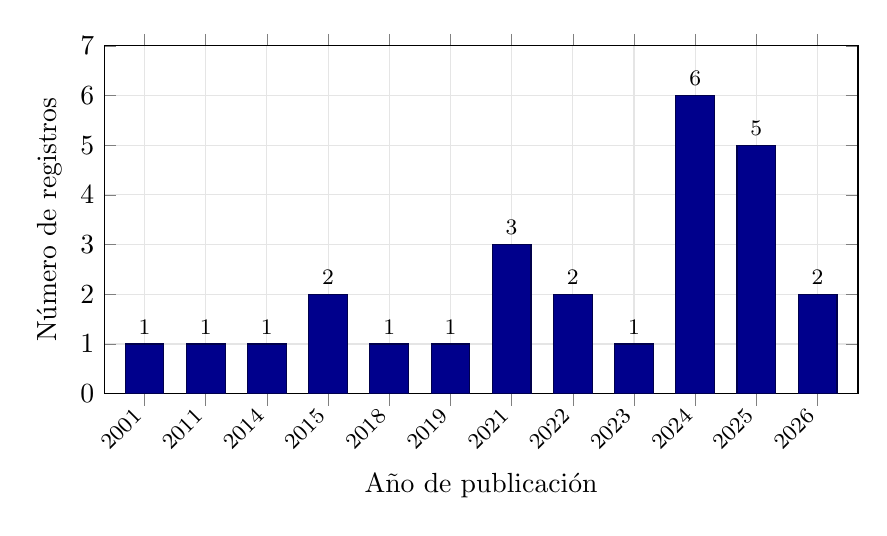
\begin{tikzpicture}
\begin{axis}[
    width=0.92\textwidth, height=6cm,
    ybar, bar width=14pt,
    ymin=0, ymax=7,
    ylabel={Número de registros},
    xlabel={Año de publicación},
    symbolic x coords={2001,2011,2014,2015,2018,2019,2021,2022,2023,2024,2025,2026},
    xtick=data,
    x tick label style={font=\footnotesize, rotate=45, anchor=east},
    ytick={0,1,2,3,4,5,6,7},
    nodes near coords, every node near coord/.append style={font=\footnotesize},
    grid=major, grid style={gray!20},
    enlarge x limits=0.06
]
\addplot[fill=blue!55!black, draw=blue!30!black] coordinates {
    (2001,1) (2011,1) (2014,1) (2015,2) (2018,1) (2019,1)
    (2021,3) (2022,2) (2023,1) (2024,6) (2025,5) (2026,2)
};
\end{axis}
\end{tikzpicture}
\caption{Distribución de los 26 registros incluidos por año de publicación.}
\label{fig:anios}
\end{figure}

La Figura~\ref{fig:anios} muestra una concentración pronunciada en el periodo
2024--2026, que reúne 13 de los 26 registros. Los antecedentes previos a 2015
corresponden en su totalidad a métodos ampelográficos y morfométricos, sin
componentes de aprendizaje automático.

\begin{figure}[htbp]
\centering
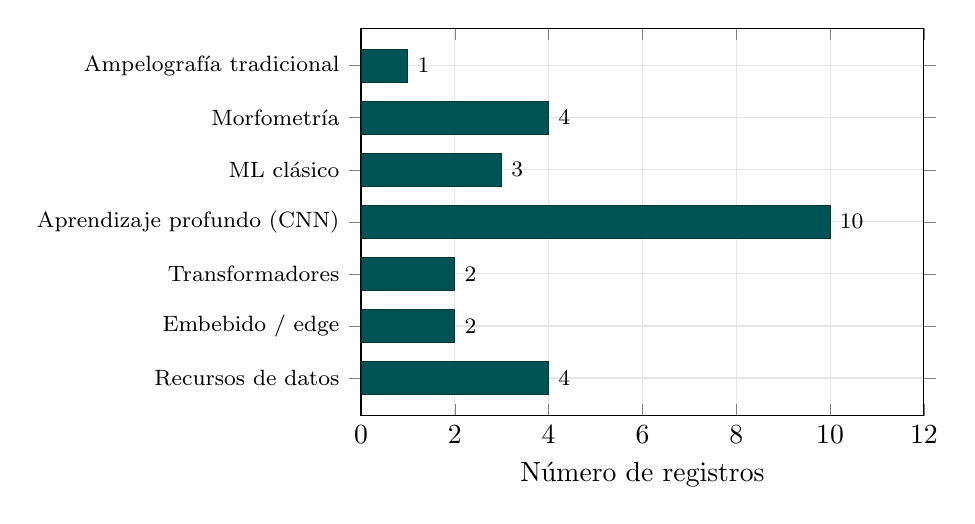
\begin{tikzpicture}
\begin{axis}[
    width=0.72\textwidth, height=6.5cm,
    xbar, bar width=12pt,
    xmin=0, xmax=12,
    xlabel={Número de registros},
    symbolic y coords={
        {Recursos de datos},
        {Embebido / edge},
        {Transformadores},
        {Aprendizaje profundo (CNN)},
        {ML clásico},
        {Morfometría},
        {Ampelografía tradicional}},
    ytick=data,
    y tick label style={font=\footnotesize},
    nodes near coords, every node near coord/.append style={font=\footnotesize},
    grid=major, grid style={gray!20},
    enlarge y limits=0.12
]
\addplot[fill=teal!65!black, draw=teal!40!black] coordinates {
    (4,{Recursos de datos})
    (2,{Embebido / edge})
    (2,{Transformadores})
    (10,{Aprendizaje profundo (CNN)})
    (3,{ML clásico})
    (4,{Morfometría})
    (1,{Ampelografía tradicional})
};
\end{axis}
\end{tikzpicture}
\caption{Frecuencia de los enfoques metodológicos identificados en la
revisión.}
\label{fig:enfoques}
\end{figure}

\begin{figure}[htbp]
\centering
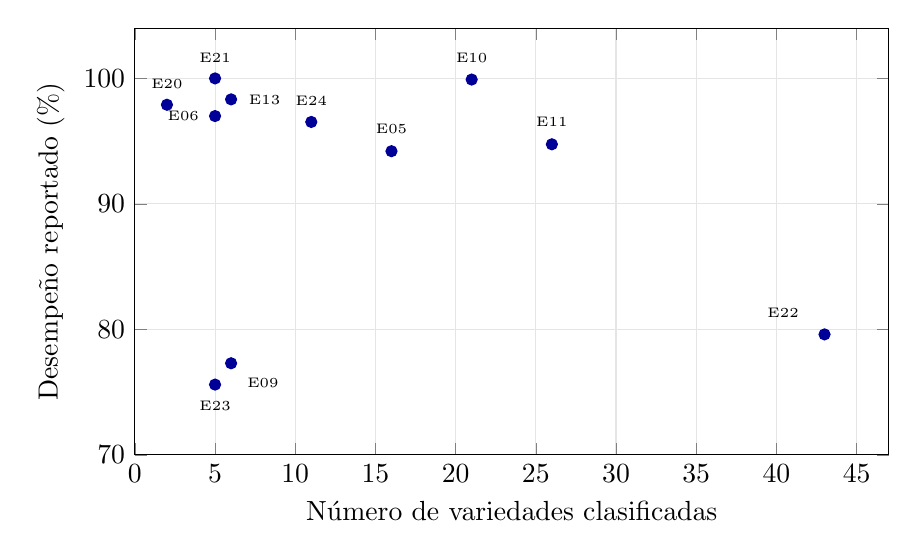
\begin{tikzpicture}
\begin{axis}[
    width=0.92\textwidth, height=7cm,
    xlabel={Número de variedades clasificadas},
    ylabel={Desempeño reportado (\%)},
    xmin=0, xmax=47,
    ymin=70, ymax=104,
    grid=major, grid style={gray!20}
]
\addplot[only marks, mark=*, mark size=2pt, color=blue!60!black]
coordinates {
    (2,97.9) (5,97.0) (5,100.0) (5,75.6) (6,77.3) (6,98.33)
    (11,96.53) (16,94.2) (21,99.91) (26,94.75) (43,79.6)
};
\node[font=\tiny, anchor=south]      at (axis cs:2,98.4)   {E20};
\node[font=\tiny, anchor=east]       at (axis cs:4.6,97.0) {E06};
\node[font=\tiny, anchor=south]      at (axis cs:5,100.5)  {E21};
\node[font=\tiny, anchor=north]      at (axis cs:5,75.1)   {E23};
\node[font=\tiny, anchor=north west] at (axis cs:6.4,76.9) {E09};
\node[font=\tiny, anchor=west]       at (axis cs:6.5,98.33){E13};
\node[font=\tiny, anchor=south]      at (axis cs:11,97.1)  {E24};
\node[font=\tiny, anchor=south]      at (axis cs:16,94.8)  {E05};
\node[font=\tiny, anchor=south]      at (axis cs:21,100.5) {E10};
\node[font=\tiny, anchor=south]      at (axis cs:26,95.4)  {E11};
\node[font=\tiny, anchor=south east] at (axis cs:42,80.2)  {E22};
\end{axis}
\end{tikzpicture}
\caption{Desempeño reportado frente al número de variedades clasificadas.
Para E20 se grafica el promedio de los dos cultivares evaluados; para E22 y
E23 se grafica el F1-score, por ser la métrica principal reportada.}
\label{fig:dispersion}
\end{figure}

La Figura~\ref{fig:dispersion} confirma la ausencia de una relación simple
entre el número de variedades y el desempeño alcanzado. Los dos valores más
bajos del corpus corresponden, por un lado, al estudio con mayor número de
clases y condiciones de adquisición más exigentes (E22, 43 variedades) y, por
otro, a un estudio con solo 5 variedades sobre un conjunto reducido (E23),
mientras que otro estudio sobre ese mismo conjunto alcanza el 100\% (E21).
Esta dispersión vertical dentro de una misma abscisa es la evidencia más
directa de que las métricas publicadas no son comparables entre sí sin
considerar el protocolo de evaluación.

\begin{figure}[htbp]
\centering
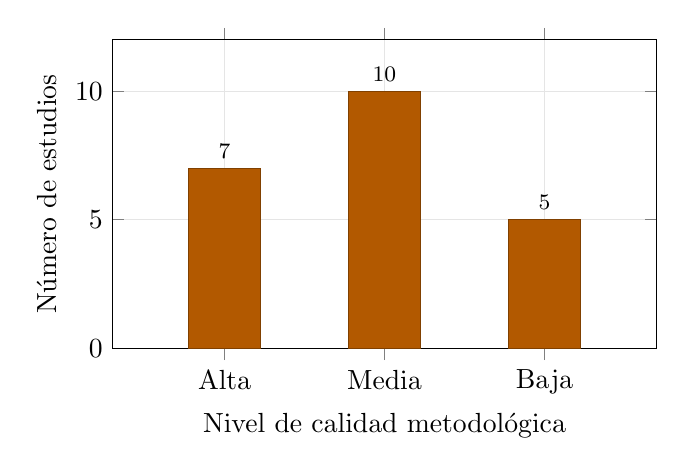
\begin{tikzpicture}
\begin{axis}[
    width=0.7\textwidth, height=5.5cm,
    ybar, bar width=26pt,
    ymin=0, ymax=12,
    ylabel={Número de estudios},
    xlabel={Nivel de calidad metodológica},
    symbolic x coords={Alta,Media,Baja},
    xtick=data,
    nodes near coords, every node near coord/.append style={font=\footnotesize},
    grid=major, grid style={gray!20},
    enlarge x limits=0.35
]
\addplot[fill=orange!70!black, draw=orange!50!black] coordinates {
    (Alta,7) (Media,10) (Baja,5)
};
\end{axis}
\end{tikzpicture}
\caption{Distribución de los 22 estudios experimentales por nivel de calidad
metodológica según la rúbrica C1--C7.}
\label{fig:calidad}
\end{figure}

\subsection{Discusión de los hallazgos}

\subsubsection{Interpretación de los resultados}

Los hallazgos revelan una tensión de tres vértices —exactitud, costo
computacional y generalización— que la literatura ha resuelto hasta ahora
sacrificando alguno de ellos. Los métodos ampelográficos y morfométricos
clásicos (E01--E04, E19) exigen recursos computacionales mínimos y ofrecen
interpretabilidad botánica directa, pero dependen de mediciones manuales que
impiden la automatización. Las redes convolucionales profundas alcanzan
exactitudes superiores al 99\% (E10) a costa de modelos de decenas de
millones de parámetros. Las arquitecturas ligeras constituyen el punto
intermedio más prometedor, y su evolución dentro del corpus es medible: de
MobileNetV2 usada como extractor de características (E06) y como clasificador
completo (E11, F1 de 94.75\% sobre 26 variedades), a una variante de
MobileNetV3-Small rediseñada específicamente para el problema, con 1.17
millones de parámetros y 96.53\% de exactitud sobre imágenes de viñedo real
(E24).

La interpretación más relevante para el presente proyecto, sin embargo, no
proviene de los valores máximos de exactitud sino de su varianza. Que E21 y
E23 reporten 100\% y 75.6\% respectivamente sobre el mismo recurso de 500
imágenes y las mismas 5 variedades indica que una parte sustancial de las
cifras publicadas mide la facilidad del conjunto de datos y no la capacidad
del modelo. Los conjuntos pequeños de fondo controlado, con particiones
aleatorias y aumento de datos aplicado antes de la partición, favorecen la
memorización de artefactos de adquisición. Esta lectura es coherente con la
caída documentada por E17 al cambiar de fuente de datos y con el F1-score de
0.796 que E22 obtiene al separar las temporadas de adquisición entre
entrenamiento y evaluación.

En cuanto a la viabilidad embebida, los estudios de identificación varietal
tratan el costo computacional como una justificación cualitativa para elegir
una arquitectura, no como una variable medida. Solo E10 valida una
implementación funcional —una aplicación Android— y solo E24 reporta el
conteo de parámetros del modelo final. Ninguno reporta latencia de
inferencia, consumo energético ni uso de memoria sobre la plataforma de
destino. Los datos más precisos sobre este eje provienen de trabajos de
detección de enfermedades: 90~ms por imagen y 3.4~W en Jetson Nano
\citep{karim2024} y 0.18~GFLOPs con 1.75 millones de parámetros
\citep{chen2025}. Esto significa que el proyecto debe importar la metodología
de medición de la literatura de enfermedades y aplicarla al problema
varietal.

\subsubsection{Comparación con otras investigaciones}

Los resultados de esta revisión coinciden con la conclusión central de las
revisiones previas sobre ampelografía digital, que identifican la
transferencia de aprendizaje sobre redes convolucionales preentrenadas como
el enfoque dominante. La aportación diferencial de la presente revisión es la
incorporación de los trabajos de 2024--2026, que modifican ese panorama en
dos sentidos: introducen los transformadores de visión y el preentrenamiento
autosupervisado como alternativa competitiva (E21, E22) y, sobre todo,
desplazan el criterio de evaluación desde la exactitud sobre conjuntos
controlados hacia la robustez en condiciones de campo (E17, E22, E24).

El antecedente local del PVVC-UABC (E19) resulta directamente consistente con
la necesidad señalada por E17 y E22 de evaluar los modelos con muestras
independientes del entrenamiento: las hojas de Misión, Syrah y Tempranillo
cultivadas en Baja California constituyen precisamente un dominio distinto al
de los conjuntos públicos europeos y turcos. Este punto adquiere mayor peso
al observar que E24 clasifica 11 cultivares que incluyen Syrah y Tempranillo,
lo que abre la posibilidad de una comparación directa entre el desempeño
publicado sobre ese conjunto chino y el desempeño obtenido sobre material
vegetal de Baja California. Se trata, en los términos de E17, de un escenario
de validación externa con variedades compartidas.

De manera complementaria, \citet{lazcano2025} (E18) —aunque enfocado en
enfermedades virales y no en identificación varietal— constituye el
antecedente regional más directo de que es viable procesar imágenes de hojas
de vid sobre plataformas de \textit{edge computing} dentro del contexto
vitivinícola de Baja California, y por tanto valida la factibilidad técnica
de la plataforma sobre la que se desplegará el sistema propuesto.

\subsubsection{Limitaciones y amenazas a la validez}

Se reconocen cinco amenazas a la validez de esta revisión.

\textbf{Cobertura incompleta de las fuentes.} La Fase~1 se ejecutó sobre
fuentes de acceso abierto y motores académicos de cobertura amplia; los
conteos exportables de Scopus, Web of Science e IEEE Xplore quedan
pendientes de la Fase~2. Es posible que existan estudios indexados
exclusivamente en esas bases que no hayan sido recuperados. La coincidencia
de 5 de los 12 registros retenidos con el conjunto documentado previamente
mitiga parcialmente esta amenaza, pero no la elimina.

\textbf{Sesgo de recuperación por acceso.} Dos informes de congreso no
pudieron evaluarse a texto completo por acceso restringido, y ambos tratan
precisamente temas centrales para las preguntas PI1 y PI5 (modelos de
conjunto y una aproximación basada en MobileNetV3Large). Su exclusión podría
subestimar la evidencia disponible sobre arquitecturas ligeras.

\textbf{Evaluación de calidad basada en información parcial.} La rúbrica
C1--C7 se aplicó a partir de los textos completos recuperados y, en los casos
en que el texto completo no estaba disponible, de resúmenes estructurados.
Las puntuaciones de E12 y E25 son las más susceptibles a esta limitación, al
haberse asignado con información reducida.

\textbf{Heterogeneidad que impide la comparación cuantitativa.} Las
diferencias en número de variedades, tamaño y procedencia de los conjuntos de
datos, estrategias de aumento, particiones y métricas hacen que las cifras de
desempeño no sean directamente comparables, motivo por el cual se descartó el
metaanálisis. Las comparaciones presentadas en la Figura~\ref{fig:dispersion}
deben leerse como una caracterización de la dispersión existente, no como un
ordenamiento de arquitecturas.

\textbf{Extracción realizada por un número reducido de revisores.} La
selección y extracción no se realizaron por duplicado de forma independiente,
por lo que no fue posible calcular un índice de concordancia entre revisores.
Esta condición introduce un riesgo de sesgo de selección que se mitigó
mediante la aplicación explícita y documentada de los criterios de
elegibilidad, pero que no queda descartado.

\subsection{Conclusiones del estado del arte}

La revisión de 26 registros confirma que la identificación automática de
variedades de vid mediante imágenes de hojas es técnicamente viable, con
exactitudes reportadas de hasta 99.91\% sobre 21 cultivares (E10), y que
existen antecedentes de implementación tanto en dispositivos móviles (E10)
como en plataformas de \textit{edge computing} en el propio contexto
vitivinícola de Baja California (E18). La evolución metodológica documentada
—de la ampelografía manual a las arquitecturas ligeras optimizadas para
campo— indica además que el problema se considera resuelto en el plano
algorítmico y que el interés de la comunidad se ha desplazado hacia las
condiciones de despliegue.

Ese desplazamiento es precisamente donde la evidencia resulta más escasa. La
evaluación de calidad muestra que 15 de los 22 estudios experimentales no
evalúan en absoluto la generalización hacia datos externos, y que solo 4
documentan los requerimientos computacionales de su modelo final. Los tres
estudios que sí abordan la generalización (E17, E22 y E24) coinciden en que
la exactitud obtenida sobre particiones aleatorias de un conjunto homogéneo
sobrestima de manera sistemática el desempeño en campo, con caídas que en el
caso de E17 resultan drásticas al cambiar de fuente de datos. A esto se suma
que ningún estudio de identificación varietal reporta latencia de inferencia,
consumo energético y exactitud medidos de forma conjunta sobre la plataforma
embebida de destino; los únicos datos precisos en ese sentido provienen de la
literatura de detección de enfermedades.

En consecuencia, ningún trabajo identificado combina simultáneamente los tres
elementos que define el presente proyecto: clasificación varietal de vid a
partir de hojas, evaluación de generalización con un conjunto local
independiente del entrenamiento, e implementación completa y caracterizada en
una plataforma embebida. Esta combinación constituye la brecha que aborda el
proyecto, y el conjunto local de Misión, Syrah y Tempranillo documentado por
el PVVC-UABC (E19) —con dos de esas tres variedades presentes también en el
conjunto de E24— ofrece la base para llevar a cabo esa evaluación externa.

% =====================================================================
\section{Problemática}
% =====================================================================

Baja California concentra la mayor parte de la producción vitivinícola del
país: de acuerdo con cifras difundidas en 2024, alrededor del 85\,\% del vino
que se produce en México proviene de este estado, que reúne más de 150
vinícolas y cerca de 4\,600 hectáreas de viñedo \citep{torres2024bc}. En una
industria de este peso regional, conocer con certeza qué variedad se tiene
plantada no es un detalle técnico: determina el manejo agronómico del
viñedo, la etiqueta del vino, el valor comercial de la uva y el cumplimiento
de los contratos entre productores y vinícolas.

A pesar de ello, la identificación varietal sigue dependiendo de dos
caminos, ambos con limitaciones importantes. El primero es la ampelografía:
la descripción morfológica de hojas, brotes y racimos por parte de un
especialista. Este método requiere personal altamente capacitado y escaso,
solo puede aplicarse en ventanas específicas del ciclo vegetativo, y su
resultado se ve afectado por la variación ambiental, las infecciones virales
que deforman la hoja, la variabilidad clonal de las variedades antiguas y la
interpretación del propio observador \citep{wineaustralia2010}. El segundo
camino es el análisis molecular mediante marcadores de ADN, que ofrece una
identificación objetiva pero exige enviar muestras a un laboratorio
especializado, con el costo y el tiempo de espera que ello implica, lo que lo
hace poco práctico como herramienta de consulta cotidiana en campo.

Las consecuencias de una identificación errónea están documentadas. En la
industria australiana se han reportado plantaciones registradas con un
nombre que en realidad contenían otra variedad, mezclas de varias
variedades bajo una sola denominación y, en el caso más conocido, un
material importado como Albariño que años después resultó ser Savagnin
Blanc, lo que obligó a reetiquetar vinos, modificar planes de
comercialización y suspender contratos con productores
\citep{wineaustralia2010}.

En el plano tecnológico, la revisión sistemática presentada en la
sección anterior muestra que la identificación automática de variedades a
partir de imágenes de hojas es técnicamente viable, con exactitudes
reportadas superiores al 95\,\% en múltiples estudios. Sin embargo, la misma
revisión evidencia dos carencias que impiden trasladar esos resultados al
campo. La primera es la falta de evaluación de la generalización: 15 de los
22 estudios experimentales no evalúan su modelo con datos externos al
conjunto de entrenamiento, y los pocos que lo hacen documentan caídas
drásticas de desempeño al cambiar la fuente de las imágenes
\citep{denart2024, carneiro2024mae}. La segunda es la falta de
caracterización embebida: ningún estudio de identificación varietal reporta
de manera conjunta la exactitud, la latencia y el consumo energético del
modelo sobre la plataforma de hardware en la que operaría.

A estas dos carencias se suma una tercera, propia del contexto regional. Los
conjuntos de datos públicos disponibles fueron adquiridos en viñedos de
Europa, Turquía y China, bajo condiciones de clima, suelo, iluminación y
equipo de captura distintas a las de Baja California. Además, la variedad
Misión —la vid histórica introducida en las misiones de la península y
genéticamente identificada con la española Listán Prieto
\citep{tapia2007}— no aparece en ninguno de los conjuntos públicos
identificados. En consecuencia, un clasificador entrenado exclusivamente con
datos públicos no solo podría perder exactitud al enfrentarse a hojas
locales de variedades conocidas, sino que tendería a asignar con falsa
seguridad una etiqueta equivocada a cualquier variedad que nunca vio durante
el entrenamiento.

Con base en lo anterior, el problema que aborda este proyecto se formula de
la siguiente manera: \textbf{no se dispone de un sistema de identificación
varietal de vid a partir de hojas que opere de forma autónoma sobre hardware
de bajo costo y cuyo desempeño haya sido verificado con hojas cultivadas en
Baja California, independientes de los datos con los que fue entrenado.}

% =====================================================================
\section{Justificación}
% =====================================================================

El desarrollo del sistema propuesto se justifica desde cuatro perspectivas.

\textbf{Relevancia regional y económica.} Dado que Baja California concentra
la mayor parte de la producción nacional de vino \citep{torres2024bc}, una
herramienta que facilite la verificación varietal atiende una necesidad
concreta de la industria local: la validación del material vegetal
adquirido en viveros, la auditoría de plantaciones existentes y la
documentación de variedades en viñedos antiguos. Un sistema embebido de
bajo costo permitiría realizar una primera verificación directamente en el
viñedo, reservando el análisis molecular —más costoso y lento— para los
casos en que el sistema reporte baja confianza o una posible discrepancia.

\textbf{Aportación técnica.} El proyecto se dirige exactamente a las dos
debilidades más marcadas que identificó la evaluación de calidad del estado
del arte: la evaluación de la generalización con datos externos (criterio
C5) y la caracterización de la viabilidad embebida (criterio C6). A
diferencia de los trabajos revisados, el sistema no se evaluará únicamente
sobre una partición del mismo conjunto con el que se entrenó, sino sobre un
conjunto local adquirido de forma independiente, y su desempeño se medirá
directamente sobre la plataforma de destino. Incorpora además un mecanismo
de rechazo por confianza, de modo que el sistema pueda reportar ``variedad
no reconocida'' en lugar de forzar una etiqueta incorrecta, una capacidad
que ninguno de los estudios revisados evalúa de forma explícita.

\textbf{Vinculación académica.} El proyecto da continuidad al trabajo del
Programa de Vinculación con Valor en Créditos de la UABC realizado en
colaboración con Viñas Pasini \citep{lopez2025pvvc}, que documentó hojas de
Misión, Syrah y Tempranillo cultivadas en Baja California. Ese material,
que por sí solo es insuficiente para entrenar una red neuronal profunda,
adquiere un valor científico particular al emplearse como conjunto de
prueba independiente, ya que permite medir de forma directa el efecto del
cambio de dominio entre los datos públicos y las condiciones locales.

\textbf{Viabilidad.} El proyecto es realizable con los recursos disponibles:
existen conjuntos de datos públicos con licencia abierta que incluyen dos de
las tres variedades locales, las arquitecturas ligeras de redes
convolucionales cuentan con modelos preentrenados de libre acceso, y las
plataformas embebidas candidatas son de bajo costo y cuentan con soporte
maduro para la ejecución de modelos cuantizados.

Los beneficiarios directos del proyecto son los productores y viveristas de
la región, que contarían con una herramienta de verificación de primer
nivel; los técnicos y enólogos, como apoyo a la labor ampelográfica; y la
comunidad académica, que dispondría de una evaluación documentada del
comportamiento de estos modelos fuera de su dominio de entrenamiento.

% =====================================================================
\section{Objetivos}
% =====================================================================

\subsection{Objetivo general}

Desarrollar e implementar un sistema embebido basado en redes neuronales
convolucionales que identifique automáticamente variedades de vid a partir
de imágenes de hojas, entrenado con conjuntos de datos públicos y validado
con un conjunto independiente de hojas cultivadas en Baja California.

\subsection{Objetivos específicos}

{\renewcommand{\labelenumi}{\textbf{OE\arabic{enumi}.}}
\begin{enumerate}
    \item Integrar un conjunto de datos de entrenamiento a partir de
    conjuntos públicos de imágenes de hojas de vid, homologando los
    sinónimos varietales y eliminando imágenes duplicadas entre fuentes.
    \item Entrenar y comparar al menos cuatro arquitecturas de redes
    neuronales convolucionales mediante transferencia de aprendizaje,
    priorizando arquitecturas ligeras, y seleccionar la de mejor equilibrio
    entre desempeño y costo computacional.
    \item Optimizar el modelo seleccionado para su ejecución en dispositivos
    con recursos limitados mediante cuantización a enteros de 8 bits,
    cuantificando la pérdida de desempeño asociada.
    \item Seleccionar la plataforma embebida de implementación mediante una
    comparación de alternativas con criterios ponderados de latencia,
    consumo energético, memoria disponible y costo.
    \item Implementar el sistema completo de captura, preprocesamiento,
    inferencia y presentación de resultados en la plataforma seleccionada,
    incluyendo un mecanismo de rechazo para variedades no reconocidas.
    \item Evaluar la capacidad de generalización del sistema con el conjunto
    local de hojas de Misión, Syrah y Tempranillo de la UABC, sin emplearlo
    en ninguna etapa de entrenamiento o ajuste.
    \item Caracterizar el desempeño del sistema sobre la plataforma
    embebida en términos de latencia de inferencia, consumo energético y uso
    de memoria.
\end{enumerate}}

% =====================================================================
\section{Hipótesis}
% =====================================================================

\textbf{Hipótesis de investigación (H1).} Un modelo de red neuronal
convolucional ligera, entrenado exclusivamente con conjuntos de datos
públicos y cuantizado a enteros de 8 bits, puede implementarse en una
plataforma embebida de bajo costo e identificar variedades de vid a partir
de imágenes de hojas con un desempeño adecuado para su uso como herramienta
de verificación en campo, aun cuando se evalúa con hojas cultivadas en Baja
California que no formaron parte del entrenamiento.

Para que la hipótesis pueda aceptarse o rechazarse de forma objetiva, se
descompone en cuatro hipótesis específicas con umbrales verificables,
resumidas en la Tabla~\ref{tab:hipotesis}. Los umbrales se fijaron a partir
de la evidencia del estado del arte: los modelos ligeros reportan entre
94.75\,\% y 96.53\,\% de exactitud en validación interna
\citep{magalhaes2023, deng2025}, por lo que un umbral de 90\,\% resulta
conservador considerando un conjunto de entrenamiento más reducido; en
cambio, los estudios que evaluaron datos externos documentan caídas
drásticas \citep{denart2024} y un F1-score de 0.796 incluso con
preentrenamiento a gran escala \citep{carneiro2024mae}, por lo que el umbral
externo se estableció en 70\,\%.

\begin{longtable}{L{1.4cm}L{6.6cm}L{5.8cm}}
\caption{Hipótesis específicas y criterios de aceptación.}
\label{tab:hipotesis} \\
\toprule
\textbf{Código} & \textbf{Hipótesis específica} & \textbf{Criterio de aceptación} \\
\midrule
\endfirsthead
\toprule
\textbf{Código} & \textbf{Hipótesis específica} & \textbf{Criterio de aceptación} \\
\midrule
\endhead
H1a & El modelo alcanza un desempeño alto dentro del dominio de los
conjuntos públicos. & Exactitud top-1 $\geq$ 90\,\% y F1-score macro
$\geq$ 0.88 en la partición de prueba interna. \\
H1b & El modelo generaliza a hojas locales de las variedades que conoce. &
Exactitud top-1 $\geq$ 70\,\% sobre las imágenes locales de Syrah y
Tempranillo. \\
H1c & El mecanismo de rechazo evita asignar etiquetas falsas a una variedad
no incluida en el entrenamiento. & Tasa de rechazo $\geq$ 70\,\% sobre las
imágenes locales de Misión. \\
H1d & El modelo optimizado es viable en la plataforma embebida sin pérdida
significativa de desempeño. & Latencia de inferencia $\leq$ 500~ms por
imagen y pérdida por cuantización $\leq$ 2 puntos porcentuales de
exactitud. \\
\bottomrule
\end{longtable}

\textbf{Hipótesis nula (H0).} Al menos uno de los criterios de la
Tabla~\ref{tab:hipotesis} no se cumple; es decir, el modelo no alcanza el
desempeño interno requerido, no generaliza a las hojas locales, no es capaz
de rechazar una variedad desconocida o no es viable sobre la plataforma
embebida seleccionada. Cada hipótesis específica se evaluará y reportará de
manera independiente, de modo que el rechazo de una de ellas documente con
precisión en qué dimensión falla el enfoque.

Las variables del estudio son las siguientes. Las \textbf{variables
independientes} son la arquitectura de la red, el esquema de optimización
(precisión completa frente a cuantización int8) y la plataforma de
ejecución. Las \textbf{variables dependientes} son la exactitud top-1, el
F1-score macro, la tasa de rechazo, la latencia de inferencia, el consumo
energético y el uso de memoria. Como \textbf{variables controladas} se
mantienen fijas la resolución de entrada, las particiones de datos y las
semillas aleatorias de entrenamiento.

% =====================================================================
\section{Metodología}
% =====================================================================

La metodología se organiza en siete etapas secuenciales, cada una con
actividades, entregables y un criterio de salida que debe cumplirse antes
de avanzar a la siguiente. La Figura~\ref{fig:metodologia} presenta el flujo
general y la Tabla~\ref{tab:etapas} resume la correspondencia entre etapas,
objetivos específicos e hipótesis.

\begin{figure}[htbp]
\centering
\begin{tikzpicture}[
    node distance=5mm and 6mm,
    etapa/.style={rectangle, draw=blue!60!black, fill=blue!8, rounded corners,
        text width=3.7cm, align=center, minimum height=1.25cm, font=\small},
    datos/.style={rectangle, draw=orange!70!black, fill=orange!10, rounded corners,
        text width=3.7cm, align=center, minimum height=1.25cm, font=\small},
    arr/.style={-{Latex[length=2mm]}, thick, draw=blue!60!black},
    darr/.style={-{Latex[length=2mm]}, thick, dashed, draw=orange!70!black}
]
\node[etapa] (e1) {\textbf{1.} Integración y curaduría de datos públicos};
\node[etapa, right=of e1] (e2) {\textbf{2.} Entrenamiento y selección de arquitectura};
\node[etapa, right=of e2] (e3) {\textbf{3.} Optimización para recursos limitados};
\node[etapa, below=of e3] (e4) {\textbf{4.} Selección de la plataforma embebida};
\node[etapa, left=of e4] (e5) {\textbf{5.} Implementación del sistema embebido};
\node[etapa, left=of e5] (e6) {\textbf{6.} Validación y caracterización};
\node[datos, below=9mm of e5] (local) {Conjunto local UABC\\(Misión, Syrah, Tempranillo)\\\footnotesize solo prueba};
\node[etapa, below=9mm of e6, fill=blue!18] (e7) {\textbf{7.} Análisis de resultados y contraste de hipótesis};

\draw[arr] (e1) -- (e2);
\draw[arr] (e2) -- (e3);
\draw[arr] (e3) -- (e4);
\draw[arr] (e4) -- (e5);
\draw[arr] (e5) -- (e6);
\draw[arr] (e6) -- (e7);
\draw[darr] (local.north west) -- (e6.south east);
\end{tikzpicture}
\caption{Flujo general de la metodología. El conjunto local de la UABC
ingresa únicamente en la etapa de validación.}
\label{fig:metodologia}
\end{figure}

\begin{longtable}{L{3.6cm}L{3.2cm}L{3.2cm}L{3.2cm}}
\caption{Correspondencia entre etapas, objetivos específicos, entregables e
hipótesis.}
\label{tab:etapas} \\
\toprule
\textbf{Etapa} & \textbf{Objetivo específico} & \textbf{Entregable} & \textbf{Hipótesis} \\
\midrule
\endfirsthead
\toprule
\textbf{Etapa} & \textbf{Objetivo específico} & \textbf{Entregable} & \textbf{Hipótesis} \\
\midrule
\endhead
1. Integración y curaduría de datos & OE1 & Conjunto integrado con particiones fijas & -- \\
2. Entrenamiento y selección & OE2 & Modelo seleccionado y tabla comparativa & H1a \\
3. Optimización & OE3 & Modelo cuantizado int8 & H1d \\
4. Selección de plataforma & OE4 & Matriz de decisión & H1d \\
5. Implementación embebida & OE5 & Prototipo funcional & -- \\
6. Validación y caracterización & OE6, OE7 & Métricas internas, externas y de hardware & H1a--H1d \\
7. Análisis de resultados & -- & Contraste de hipótesis & H1, H0 \\
\bottomrule
\end{longtable}

\subsection{Etapa 1: Integración y curaduría de datos públicos}

El conjunto de entrenamiento se construirá a partir de conjuntos públicos
con licencia abierta. La base principal será GLVD \citep{glvd2026}, que
compila 1\,469 imágenes de 16 cultivares con particiones predefinidas e
integra los recursos de \citet{koklu2022dataset} y \citet{vlah2021}; se
complementará con el UTAD Grapevine Varieties Dataset 2023
\citep{utad2024}, que aporta imágenes adquiridas con nueve dispositivos
distintos y mayor variabilidad de condiciones. El conjunto INCAFO
\citep{incafo2023}, con 37 variedades, se solicitará a sus autores dado que
su acceso es restringido; su incorporación se considerará opcional.

La Tabla~\ref{tab:cobertura} muestra la cobertura de las tres variedades
locales en los conjuntos públicos identificados. Syrah y Tempranillo están
disponibles en al menos un conjunto abierto; Misión no aparece en ninguno.
Esta condición define el diseño experimental de la validación: Syrah y
Tempranillo funcionarán como clases conocidas para medir la generalización
(H1b), mientras que Misión funcionará como variedad desconocida para medir
la capacidad de rechazo del sistema (H1c).

\begin{longtable}{L{2.6cm}L{3.8cm}L{2.2cm}L{2.2cm}L{2.2cm}}
\caption{Cobertura de las variedades locales en los conjuntos públicos.}
\label{tab:cobertura} \\
\toprule
\textbf{Variedad local} & \textbf{Sinónimos} & \textbf{GLVD / Kaggle} & \textbf{UTAD 2023} & \textbf{INCAFO} \\
\midrule
\endfirsthead
\toprule
\textbf{Variedad local} & \textbf{Sinónimos} & \textbf{GLVD / Kaggle} & \textbf{UTAD 2023} & \textbf{INCAFO} \\
\midrule
\endhead
Syrah & Shiraz & Sí & No & Sí \\
Tempranillo & Tinta Roriz, Aragonez & Sí & Sí (Tinta Roriz) & Sí (Aragonez) \\
Misión & Listán Prieto, País, Criolla Chica & No & No & No \\
\midrule
\multicolumn{2}{l}{Licencia} & CC BY 4.0 & CC BY 4.0 & Restringida \\
\bottomrule
\end{longtable}

Las actividades de esta etapa son: (a) homologar las etiquetas de las
distintas fuentes, unificando sinónimos varietales bajo un solo nombre;
(b) eliminar imágenes duplicadas o casi duplicadas mediante comparación por
\textit{hash} perceptual, paso indispensable porque GLVD integra imágenes
de otros conjuntos públicos y un duplicado presente en entrenamiento y en
prueba inflaría artificialmente las métricas; (c) excluir las clases con
un número insuficiente de imágenes; y (d) generar particiones estratificadas
de entrenamiento, validación y prueba, que quedarán fijas para todo el
proyecto. El criterio de salida es disponer del conjunto integrado, con sus
particiones congeladas y un reporte del número de imágenes por clase.

\subsection{Etapa 2: Entrenamiento y selección de arquitectura}

Se entrenarán al menos cuatro arquitecturas mediante transferencia de
aprendizaje a partir de pesos preentrenados en ImageNet: MobileNetV2,
MobileNetV3-Small y EfficientNet-B0 como candidatas ligeras, y ResNet-50
como referencia de mayor capacidad. El entrenamiento se realizará en dos
fases: primero con la base convolucional congelada para ajustar el
clasificador, y después con descongelamiento parcial de las capas
superiores y una tasa de aprendizaje reducida.

Las imágenes se redimensionarán a $224\times224$ píxeles y se normalizarán
según los parámetros de ImageNet. El aumento de datos —rotaciones,
reflejos, variaciones de brillo, contraste y tono, y recortes aleatorios—
se aplicará exclusivamente sobre la partición de entrenamiento y después de
generar las particiones. Esta precaución responde directamente a la
evidencia del estado del arte, donde dos estudios sobre el mismo conjunto
reportan desempeños separados por casi 25 puntos porcentuales
\citep{kunduracioglu2024, huang2025}.

Cada arquitectura se entrenará con tres semillas aleatorias distintas y se
reportará la media y la desviación estándar de la exactitud top-1 y del
F1-score macro sobre la partición de prueba interna, junto con la matriz
de confusión. La arquitectura se seleccionará con un criterio de
equilibrio: entre los modelos que cumplan el umbral de H1a, se elegirá el de
menor número de parámetros y operaciones de punto flotante.

\subsection{Etapa 3: Optimización para recursos limitados}

El modelo seleccionado se convertirá a un formato de inferencia embebida
(TensorFlow Lite u ONNX, según la plataforma) y se aplicará cuantización
posterior al entrenamiento a enteros de 8 bits, utilizando un subconjunto
representativo de la partición de entrenamiento para la calibración. Se
medirá el tamaño del modelo y la exactitud antes y después de la
cuantización sobre la misma partición de prueba. Si la pérdida supera el
umbral de H1d, se aplicará entrenamiento consciente de la cuantización
como alternativa.

En esta etapa se fijará también el umbral del mecanismo de rechazo. Se
utilizará la probabilidad máxima de la salida \textit{softmax} como medida
de confianza, y el umbral se calibrará sobre la partición de validación de
los conjuntos públicos, de manera que acepte al menos el 95\,\% de las
predicciones correctas. El umbral quedará fijo antes de cualquier contacto
con el conjunto local, para que la evaluación de H1c no esté sesgada.

\subsection{Etapa 4: Selección de la plataforma embebida}

La plataforma de implementación se seleccionará mediante una matriz de
decisión ponderada entre tres alternativas representativas de distintos
niveles de capacidad y costo: una computadora de placa única basada en CPU
(Raspberry Pi 5), un módulo con aceleración por GPU (NVIDIA Jetson Orin
Nano) y un microcontrolador con cámara integrada (ESP32-S3). Los criterios
de evaluación serán la latencia de inferencia del modelo cuantizado, el
consumo energético, la memoria disponible frente a la requerida por el
modelo, el costo de adquisición y la madurez del soporte de software y de
cámara. Como filtro previo se descartará cualquier plataforma en la que el
modelo no quepa en memoria o no alcance el umbral de latencia de H1d. El
entregable de la etapa es la matriz de decisión con la justificación de la
plataforma elegida.

\subsection{Etapa 5: Implementación del sistema embebido}

Sobre la plataforma seleccionada se implementará el flujo completo del
sistema: captura de la imagen de la hoja mediante la cámara,
preprocesamiento con los mismos parámetros empleados en el entrenamiento,
inferencia con el modelo cuantizado, aplicación del umbral de rechazo y
presentación del resultado al usuario, incluyendo la variedad identificada
—o la indicación de ``variedad no reconocida''— y el nivel de confianza
asociado. El criterio de salida es un prototipo que ejecute el flujo
completo de forma autónoma, sin depender de una computadora externa ni de
conexión a internet.

\subsection{Etapa 6: Validación y caracterización}

La validación se realizará en tres niveles. El \textbf{nivel interno}
evaluará el modelo sobre la partición de prueba de los conjuntos públicos
para contrastar H1a. El \textbf{nivel externo} evaluará el sistema sobre el
conjunto local de la UABC: las imágenes de Syrah y Tempranillo se usarán
para medir la exactitud top-1 (H1b) y las de Misión para medir la tasa de
rechazo (H1c). El conjunto local no se utilizará en ninguna etapa de
entrenamiento, selección de arquitectura, calibración del umbral ni ajuste
de hiperparámetros. Dado que el conjunto local es de tamaño reducido, las
métricas externas se reportarán acompañadas de intervalos de confianza al
95\,\% calculados con el método de Wilson, para que la aceptación o rechazo
de la hipótesis considere la incertidumbre asociada al tamaño de muestra.

El \textbf{nivel de hardware} caracterizará el sistema sobre la plataforma
embebida: latencia de inferencia (media y percentil 95 sobre al menos 100
ejecuciones, excluyendo las ejecuciones iniciales de calentamiento),
consumo energético durante la inferencia medido con un medidor de
potencia en la alimentación, y uso máximo de memoria. Estas mediciones
permitirán contrastar H1d.

\subsection{Etapa 7: Análisis de resultados y contraste de hipótesis}

Cada hipótesis específica se contrastará contra su criterio de aceptación y
se reportará de manera independiente. Se analizarán además las matrices de
confusión internas y externas para identificar qué variedades se confunden
con mayor frecuencia, y se compararán los resultados con los reportados en
el estado del arte, con especial atención a la magnitud de la caída entre
la evaluación interna y la externa. En caso de que alguna hipótesis se
rechace, el análisis documentará la causa probable —insuficiencia de datos,
cambio de dominio o limitación del hardware— como base para trabajos
futuros.

\subsection{Alcance y limitaciones}

El sistema se limita a la identificación de variedades a partir de hojas
maduras fotografiadas individualmente; no contempla racimos, sarmientos ni
la detección de enfermedades. El número de variedades que el sistema podrá
reconocer está determinado por la cobertura de los conjuntos públicos, por
lo que Misión no podrá identificarse positivamente sino únicamente
rechazarse como variedad desconocida. Los resultados de la validación
externa corresponden a las condiciones de captura del conjunto local de la
UABC y no deben extrapolarse sin evaluación adicional a otros viñedos,
temporadas o dispositivos de captura. Finalmente, el sistema se plantea como
una herramienta de verificación de primer nivel y no sustituye al análisis
molecular en los casos que requieran certeza legal o comercial.
